\section{Capitulo 3: Selección del mecanismo de integración y herramienta LLM}
\label{seleccionllm}

Con la arquitectura UNS implementada (Capítulo 2), el siguiente paso consiste en definir cómo se conecta un modelo de lenguaje de gran tamaño (LLM) a esa estructura de datos. Esta decisión tiene dos partes: primero, qué mecanismo de comunicación usar entre el UNS y el LLM; segundo, qué herramienta LLM emplear. Este capítulo desarrolla ambos aspectos, siguiendo el análisis comparativo documentado que exige la propuesta de este trabajo.

\subsection{Mecanismos de integración de LLM con sistemas externos en IIoT}
\label{mecanismosintegracion}

Conectar un LLM a una fuente de datos externa no es un problema nuevo, pero sí lo es hacerlo en un contexto industrial donde la fuente cambia constantemente de valor y donde una mala configuración puede exponer información sensible del proceso. La literatura y la práctica de la industria coinciden en tres formas de resolver esta conexión: invocación directa mediante HTTP/REST, orquestación mediante pipelines de procesamiento, y Model Context Protocol (MCP) \cite{MastouriRESTtoMCP2026, EhteshamAgentProtocols2025}. Las tres se describen a continuación de forma general, antes de compararlas frente al caso de estudio en la Sección \ref{analisiscomparativo}.

\subsubsection{Invocación directa mediante HTTP/REST}

REST (\textit{Representational State Transfer}) es un estilo arquitectónico para sistemas distribuidos, no un protocolo en sí mismo \cite{ReSTFielding2000}. Se apoya sobre HTTP y define un conjunto de restricciones: interfaz uniforme, recursos identificables mediante URI, y comunicación sin estado, donde cada petición contiene toda la información necesaria para procesarla, sin depender de peticiones anteriores.

Aplicado a la integración de un LLM con una fuente de datos industrial, este enfoque implica exponer los datos del UNS como un conjunto de \textit{endpoints} (por ejemplo, \texttt{GET /linea/A/oee}), que el LLM invoca mediante peticiones HTTP explícitas. El desarrollador debe programar de antemano cuál endpoint corresponde a determinada consulta, ya que el LLM no tiene forma nativa de descubrir en tiempo de ejecución qué recursos existen ni qué significan. Cada nueva fuente de datos (una línea adicional, un nuevo sistema ERP) exige escribir y mantener el conector correspondiente. Este patrón de integración ad hoc, repetido por cada combinación de modelo y fuente de datos, es lo que en la industria se conoce como el problema de los conectores fragmentados \cite{anthropic2024intro}.

\subsubsection{Orquestación mediante pipelines de procesamiento}

Un segundo enfoque introduce una capa intermedia entre el LLM y las fuentes de datos: un motor de orquestación que define, paso a paso, cómo se recupera, transforma y entrega la información al modelo. A diferencia de la invocación directa, aquí el LLM no llama a la fuente de datos por sí mismo; el pipeline decide qué pasos ejecutar, en qué orden y con qué transformaciones intermedias, y solo entrega al LLM el resultado ya procesado.

Este patrón es común en frameworks de orquestación de agentes, donde cada paso del pipeline puede invocar una API distinta, aplicar una regla de negocio o enriquecer el dato con contexto adicional antes del siguiente paso \cite{EhteshamAgentProtocols2025}. La ventaja operativa se tiene el control explícito sobre el flujo de datos, mientras que como desventaja se tiene que el control depende enteramente de cómo se configuró el pipeline: agregar una nueva fuente o un nuevo tipo de consulta no es tan simple como registrar un endpoint, sino que exige modificar la lógica del pipeline mismo.

\subsubsection{Model Context Protocol (MCP)}

MCP es un estándar abierto introducido por Anthropic a finales de 2024, diseñado para conectar asistentes de IA con las fuentes de datos y herramientas externas donde reside la información \cite{anthropic2024intro}. A diferencia de los dos mecanismos anteriores, MCP no fue diseñado pensando en un desarrollador que programa una integración, sino en un modelo de lenguaje que necesita descubrir, en tiempo de ejecución, qué herramientas y datos tiene disponibles.

Su arquitectura sigue un modelo cliente-servidor: una aplicación de IA actúa como anfitrión MCP y se conecta a uno o más servidores MCP mediante clientes dedicados, cada uno con una conexión independiente \cite{anthropic2024arch}. La comunicación se organiza en dos capas: una capa de datos basada en JSON-RPC 2.0, que define la negociación de capacidades y la exposición de funcionalidades del servidor, y una capa de transporte que gestiona la conexión y la autenticación, ya sea local (STDIO) o remota (HTTP, con soporte para OAuth) \cite{anthropic2024arch}.

El concepto central son las primitivas de contexto que el servidor expone al cliente: \textit{Tools} (funciones ejecutables, como consultar un tag o disparar una acción), \textit{Resources} (fuentes de datos con contexto estructurado) y \textit{Prompts} (plantillas reutilizables) \cite{anthropic2024arch}. Sobre esta base, MCP también incorpora un sistema de notificaciones al que el cliente puede suscribirse para mantenerse sincronizado con cambios en el servidor, evitando así las consultas repetidas propias de otros mecanismos.

% TODO-FIGURA 1
\begin{figure}[H]
\centering
 \centerline{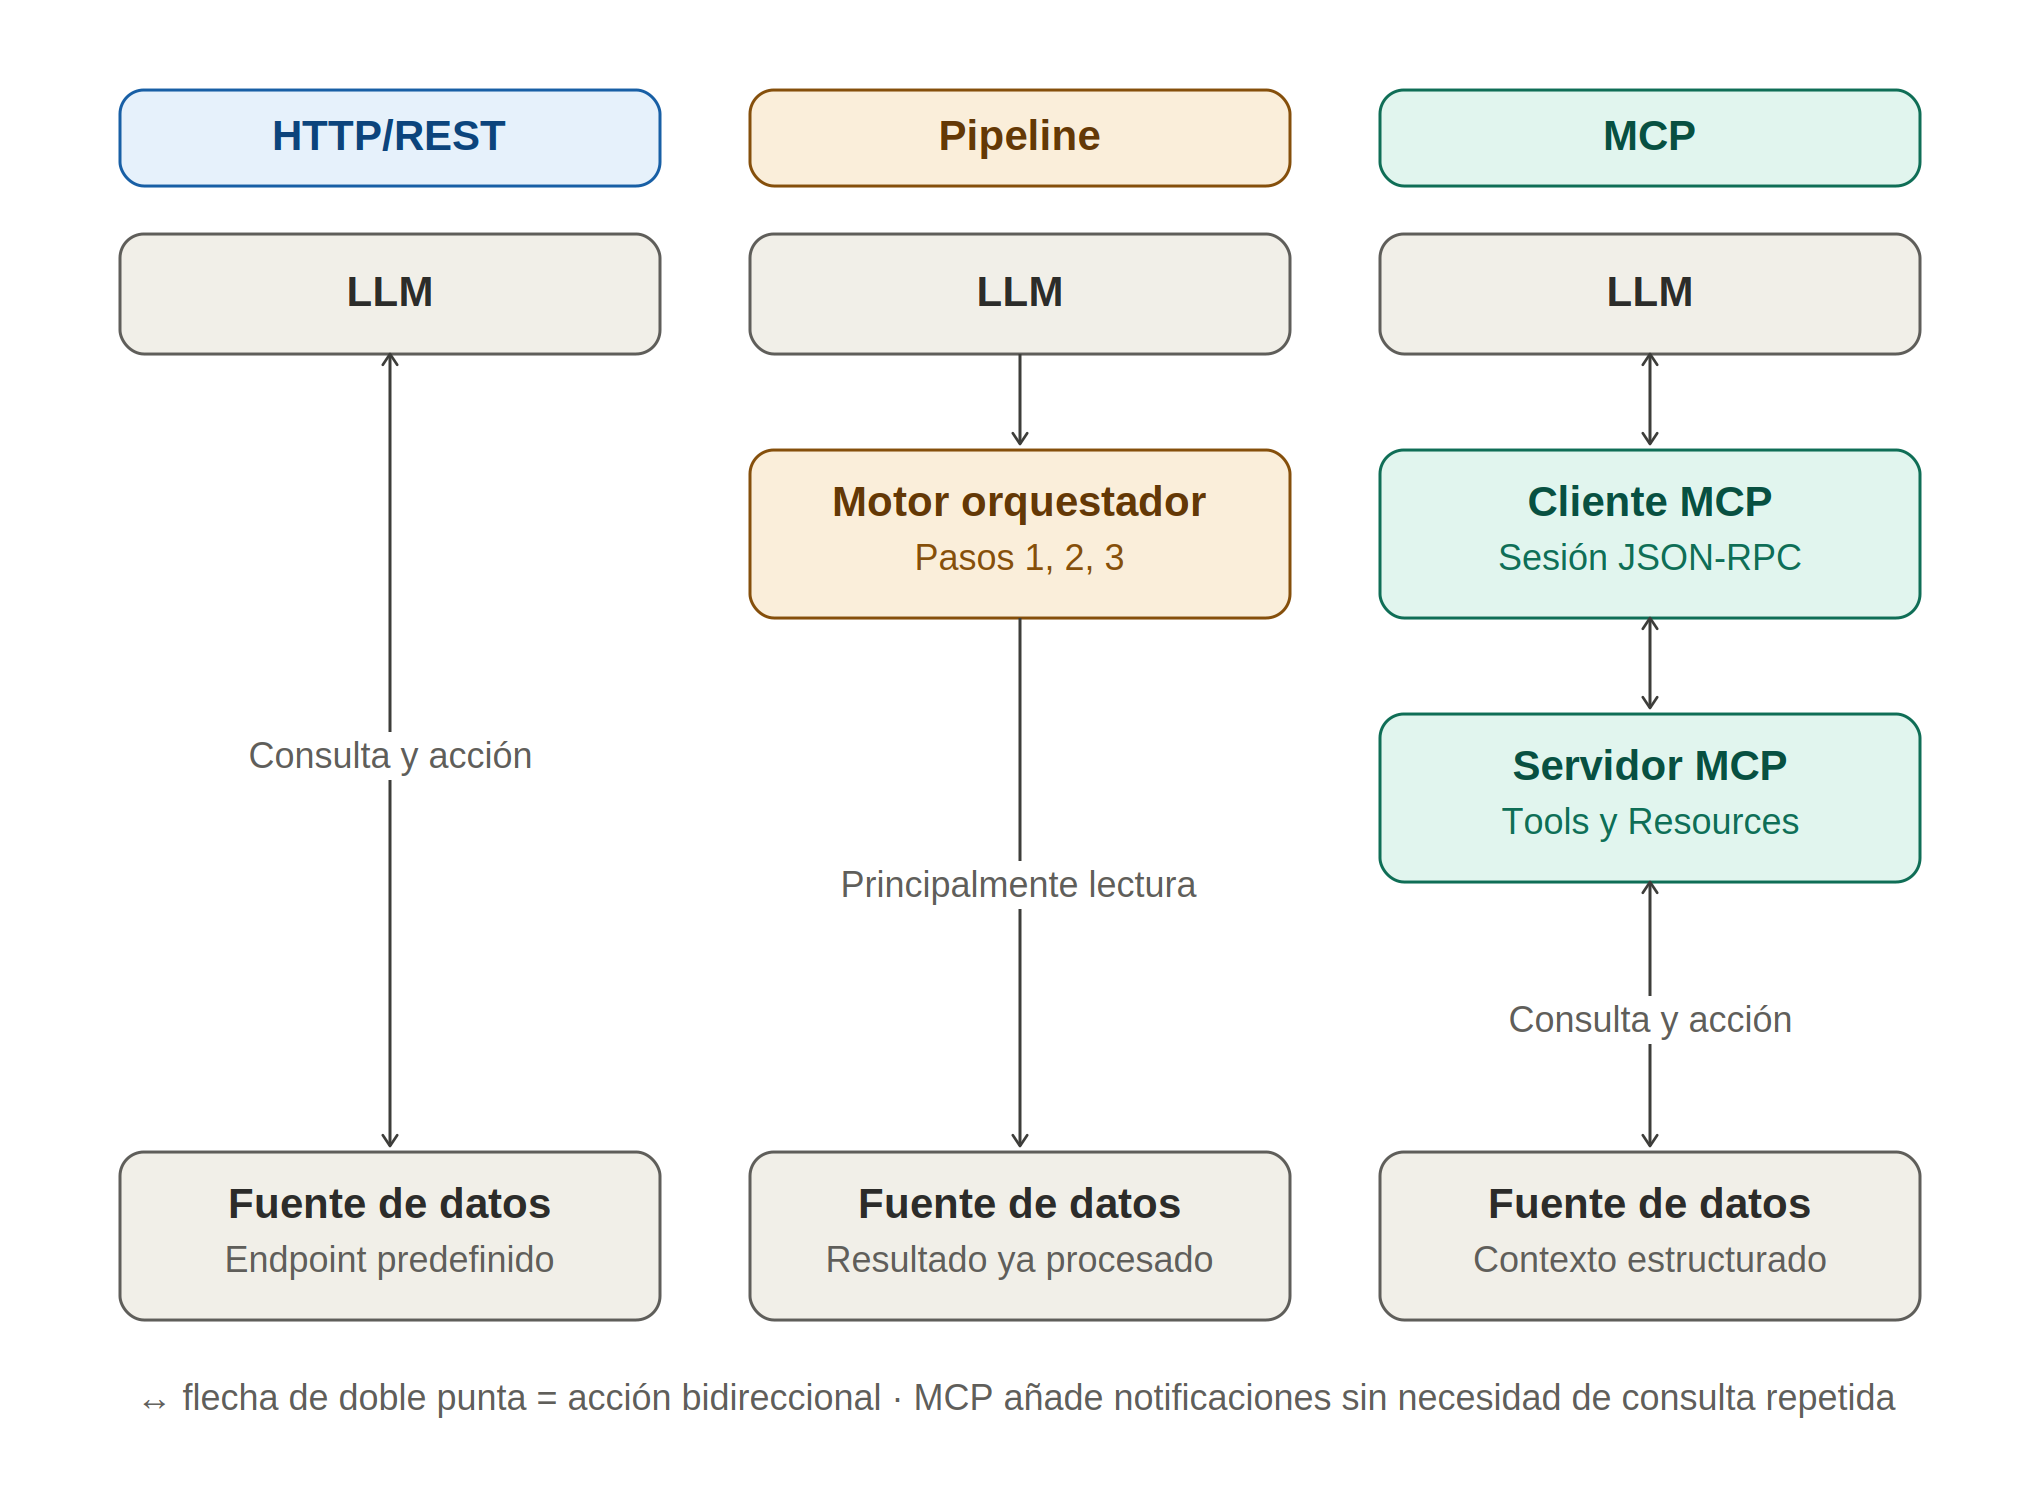
\includegraphics[width=13cm]{Figuras/mecanismos_integracion.png}}
\caption{Comparación esquemática de los mecanismos de integración LLM-UNS: HTTP/REST, pipeline de orquestación y MCP. Elaboración propia.}
\label{fig:mecanismos_integracion}
\end{figure}


\subsection{Criterios de comparación}
\label{criterioscomparacion}

Comparar estos tres mecanismos exige criterios concretos, no una preferencia general por lo más reciente o lo más popular. Se definieron seis criterios, anclados a tres fuentes distintas: los tres primeros provienen textualmente de la justificación de la propuesta de este trabajo; el cuarto y el quinto se derivan de los requerimientos funcionales identificados en la caracterización del caso de estudio (Capítulo 1, R1 y R2/R3); el sexto es un criterio técnico complementario, sin anclaje directo en la propuesta, incluido por buenas prácticas de arquitectura de software.

\begin{enumerate}
    \item \textbf{Acceso a variables en tiempo real} (propuesta). Mide si el mecanismo permite consultar el estado actual del proceso sin latencia significativa ni pasos intermedios de sincronización.
    \item \textbf{Acción bidireccional} (propuesta). Mide si el mecanismo permite no solo leer datos del UNS, sino también escribir o ejecutar acciones sobre el sistema.
    \item \textbf{Restricciones de privacidad IIoT} (propuesta). Mide la granularidad del control de acceso y la madurez de los mecanismos de autenticación y autorización propios del mecanismo.
    \item \textbf{Capacidad de exponer contexto semántico} (R1). Mide si el mecanismo transmite al LLM el significado del dato (jerarquía, unidades, procedencia), no solo su valor crudo.
    \item \textbf{Esfuerzo de desarrollo y mantenimiento} (R2/R3). Mide cuánto código a la medida hay que escribir y sostener para conectar cada fuente de datos del UNS.
    \item \textbf{Interoperabilidad multi-proveedor} (técnico). Mide el grado de acoplamiento de la solución a un único proveedor de LLM.
\end{enumerate}

\subsection{Análisis comparativo de los mecanismos de integración}
\label{analisiscomparativo}

La Tabla \ref{tab:comparacion_mecanismos} resume la evaluación de los tres mecanismos frente a los seis criterios definidos. La calificación usa tres niveles: \checkmark\checkmark~(cumple de forma robusta), \checkmark~(cumple de forma parcial o requiere trabajo adicional) y \texttimes~(no cumple o presenta una limitación significativa).

\begin{table}[H]
\centering
\caption{Comparación de mecanismos de integración LLM-UNS frente a los seis criterios definidos.}
\label{tab:comparacion_mecanismos}
\begin{tabular}{p{4.3cm}ccc}
\hline
\textbf{Criterio} & \textbf{HTTP/REST} & \textbf{Pipelines} & \textbf{MCP} \\
\hline
Acceso en tiempo real & \checkmark & \texttimes & \checkmark\checkmark \\
Acción bidireccional & \checkmark & \texttimes & \checkmark\checkmark \\
Privacidad IIoT & \checkmark\checkmark & \checkmark & \texttimes \\
Contexto semántico & \texttimes & \checkmark & \checkmark\checkmark \\
Esfuerzo de desarrollo & \texttimes & \texttimes & \checkmark\checkmark \\
Interoperabilidad multi-proveedor & \checkmark & \texttimes & \checkmark\checkmark \\
\hline
\end{tabular}
\end{table}

\textbf{Acceso a variables en tiempo real.} HTTP/REST permite lectura bajo demanda, pero depende de que el cliente pregunte (\textit{polling}); no hay un mecanismo nativo para que el servidor avise de un cambio. Los pipelines de orquestación añaden latencia adicional por las etapas intermedias de procesamiento, lo que los deja en la posición más débil de los tres. MCP resuelve esto mediante suscripción, su sistema de notificaciones mantiene al cliente sincronizado sin necesidad de consultas repetidas \cite{anthropic2024arch}, lo que se traduce en acceso inmediato al estado del proceso, tal como demuestran Yang et al. en su implementación de MCP sobre sistemas IoT industriales \cite{YangIoTMCP2025}.

\textbf{Acción bidireccional.} REST soporta lectura y escritura a nivel de protocolo (GET, POST, PUT), pero el LLM necesita saber de antemano cuál endpoint invocar para cada acción, sin mecanismo de descubrimiento. Los pipelines suelen diseñarse para flujos de lectura y transformación; añadir escritura implica construir pasos adicionales de forma explícita. MCP fue diseñado desde el inicio para conexiones bidireccionales entre la aplicación de IA y las fuentes externas \cite{anthropic2024intro}, con la ventaja adicional de que la acción queda descrita junto con su contexto semántico dentro del bloque primitivo \textit{Tool}.

\textbf{Restricciones de privacidad IIoT.} Este es el único criterio donde REST aventaja claramente a los otros dos. Sus mecanismos de autenticación y autorización (OAuth2, API keys) son robustos y han sido ampliamente usados en auditoría en producción. MCP, al ser una tecnología emergente, presenta una superficie de ataque documentada: Hou et al. identifican dieciséis escenarios de amenaza distribuidos en las cuatro fases del ciclo de vida de un servidor MCP, incluyendo envenenamiento de herramientas y ejecución remota no autorizada \cite{HouMCPLandscape2025}. Los pipelines de orquestación quedan en una posición intermedia: su seguridad depende enteramente de cómo se implementó el motor de orquestación, sin un estándar unificado que la respalde.

\textbf{Capacidad de exponer contexto semántico.} La respuesta de un endpoint REST es, por diseño, un valor sin contexto adicional; el significado de ese valor vive en la documentación externa que el LLM no consulta durante la ejecución. Un pipeline puede enriquecer el dato en sus etapas intermedias, pero solo si alguien diseñó esa etapa explícitamente. El bloque primitivo \textit{Resources} de MCP resuelve este problema de forma estructural, al exponer no solo el dato sino su procedencia dentro de la jerarquía del servidor \cite{anthropic2024arch}. La revisión sistemática de Abu-Salih et al. sobre el uso de LLM para interoperabilidad semántica confirma que este tipo de exposición estructurada de contexto es, hasta ahora, el factor que más impacta la calidad de las respuestas de un LLM sobre datos heterogéneos \cite{AbuSalihSemanticLLM2025}.

\textbf{Esfuerzo de desarrollo y mantenimiento.} REST exige un conector a la medida por cada fuente de datos del UNS; los pipelines suman a ese esfuerzo el mantenimiento del propio motor de orquestación, lo que los ubica como la opción más costosa de sostener en el tiempo. MCP invierte esta lógica: en lugar de construir un conector por combinación de modelo y fuente, se construye un servidor MCP una sola vez, reutilizable por cualquier cliente compatible \cite{AhmadiMCPBridge2025}. El estudio presentado por Chen et al., basado en entrevistas con veinte profesionales de ocho empresas, confirma que la reducción de conectores a la medida es, en la práctica, el beneficio que más valoran los equipos que adoptan MCP en flujos de trabajo con LLM \cite{ChenEnterpriseMCP2026}.

\textbf{Interoperabilidad multi-proveedor.} REST es neutral por diseño: cualquier LLM puede invocar un endpoint REST si se le programa la lógica correspondiente, aunque esa lógica deba reescribirse para cada proveedor. Los pipelines suelen depender del framework de orquestación elegido, lo que introduce un acoplamiento adicional no siempre compatible con distintos proveedores de LLM. MCP, al ser un estándar abierto, ha sido adoptado como protocolo de host por múltiples proveedores más allá de Anthropic \cite{EhteshamAgentProtocols2025}, lo que reduce el riesgo de atar la arquitectura del caso de estudio a una única herramienta LLM.

El balance final es de cinco criterios a favor de MCP y uno a favor de HTTP/REST. Vale la pena señalar que este resultado no oculta una limitación real de MCP: el criterio donde pierde, privacidad, no es menor en un contexto industrial, y se retoma en la sección siguiente como parte de la decisión, no como una nota al margen.

\subsection{Selección del mecanismo de integración}
\label{seleccionmecanismo}

Con base en el análisis de la Sección \ref{analisiscomparativo}, se selecciona MCP como mecanismo de integración entre el LLM y la arquitectura UNS del caso de estudio. La decisión se apoya en que las prioridades del caso de estudio (acceso a datos de producción en tiempo real, capacidad de que el LLM actúe sobre el sistema, y necesidad de exponer contexto semántico de una jerarquía de datos compleja) coinciden exactamente con los criterios donde MCP demostró ventaja.

La brecha en privacidad no se ignora. Dado que MCP aún no iguala la madurez de REST en control de acceso, esta limitación se reconoce como un riesgo aceptado en esta fase de selección del mecanismo, que deberá abordarse durante la implementación de la integración sobre el caso de estudio (Capítulo 4), en vez de resolverse aquí con una medida que el análisis comparativo no sustentó.

Como referencia para esa implementación, tres decisiones de diseño concretas pueden reducir esa brecha sin necesidad de mecanismos ajenos al protocolo: adoptar transporte STDIO en lugar de HTTP remoto, dado que el servidor Ignition del caso de estudio es local y no requiere exposición de red; limitar el alcance del servidor MCP a herramientas de lectura sobre los contextos MES, Line, ERP y Edge ya definidos en el Capítulo 2, sin incluir operaciones de escritura ni acceso a la configuración interna de Ignition; y, si en el futuro se requiere un transporte remoto, exigir autenticación OAuth en esa capa, tal como lo contempla la especificación del protocolo \cite{anthropic2024arch}.

% TODO-FIGURA 2
\begin{figure}[H]
\centering
 \centerline{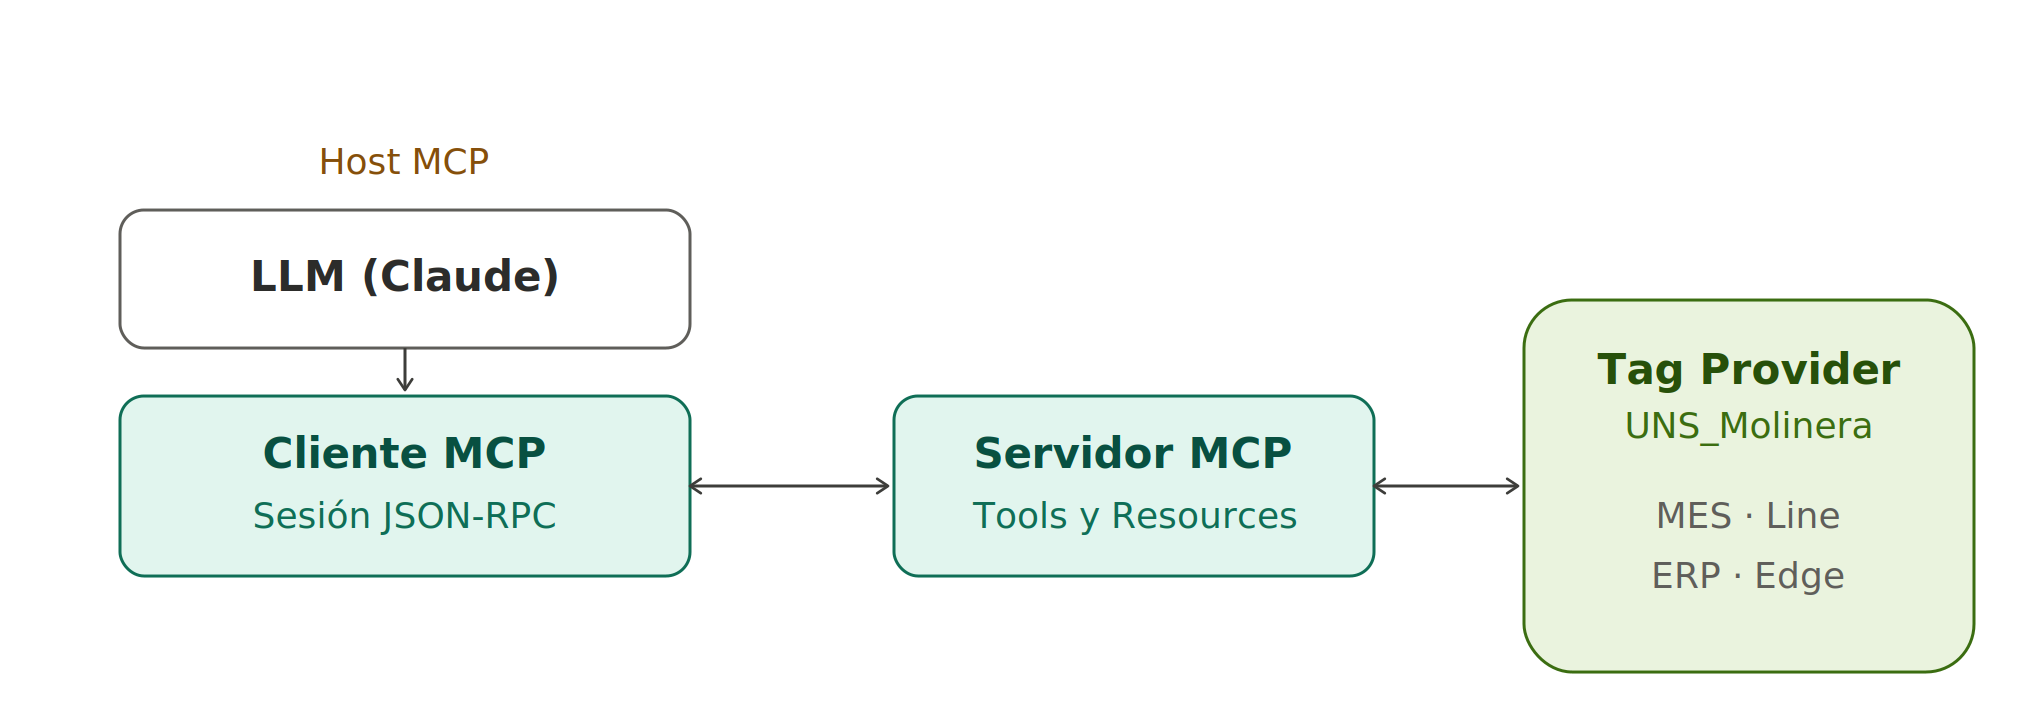
\includegraphics[width=15cm]{Figuras/mcp_uns.png}}
\caption{Arquitectura de integración seleccionada: servidor MCP entre el LLM y el Tag Provider \texttt{UNS\_Molinera}. Elaboración propia.}
\label{fig:mcp_lista_blanca}
\end{figure}

La Figura \ref{fig:mcp_lista_blanca} resume el flujo de una consulta típica. Cuando el LLM necesita un dato, el Cliente MCP invoca al Servidor MCP a través de la conexión establecida, especificando la herramienta y los parámetros correspondientes. El Servidor MCP traduce esa invocación en una lectura sobre el Tag Provider \texttt{UNS\_Molinera}, y devuelve el resultado ya estructurado con su contexto (a qué línea, a qué corrida y a qué unidad de medida corresponde), no solo el valor crudo. Cuando una pregunta requiere combinar más de un contexto de datos (por ejemplo, cruzar el contexto ERP con el MES para responder si una línea va atrasada respecto a su meta), este ciclo de invocación y respuesta se repite tantas veces como sea necesario antes de que el LLM redacte la respuesta final, sin que el operador tenga que descomponer la pregunta en pasos.

\subsection{Selección de la herramienta LLM}
\label{seleccionherramientallm}

\subsubsection{Criterios de adaptabilidad al caso de estudio}

Definido el mecanismo de integración, la elección de la herramienta LLM se evalúa contra tres criterios de adaptabilidad al caso de estudio, distintos de los seis usados para comparar mecanismos, porque aquí la pregunta ya no es qué protocolo usar sino qué modelo aprovecha mejor ese protocolo.

El primero es el soporte nativo del protocolo MCP como anfitrión (\textit{host}), sin requerir adaptadores intermedios que traduzcan entre el modelo y el servidor MCP. El segundo es la capacidad de razonamiento necesaria para encadenar múltiples invocaciones de herramientas y sintetizar resultados de distintas fuentes en una sola respuesta coherente, capacidad que la literatura sobre agentes basados en LLM describe como el patrón de intercalar razonamiento y acción en pasos sucesivos \cite{YaoReAct2023}. El tercero es la capacidad de interpretar y mapear terminología técnica del dominio industrial a las variables correspondientes de la jerarquía UNS, de modo que una pregunta formulada en lenguaje natural por un operador se traduzca correctamente en la ruta de tags adecuada.

\subsubsection{Selección de Claude (Anthropic)}

Se selecciona Claude (Anthropic) como herramienta LLM para este trabajo. La justificación sigue los tres criterios anteriores.

Sobre soporte nativo de MCP, Claude fue el primer anfitrión de referencia del protocolo, dado que Anthropic es su creador y mantiene la especificación oficial \cite{anthropic2024arch}; esto elimina la necesidad de un adaptador intermedio entre el modelo y el servidor MCP construido para el caso de estudio.

Sobre capacidad de razonamiento para encadenar herramientas, Claude sostiene conversaciones donde una sola consulta del operador puede requerir varias invocaciones sucesivas al servidor MCP (por ejemplo, leer el estado de la línea, cruzarlo con la orden de producción activa, y solo entonces responder), sin que el operador tenga que descomponer la pregunta en pasos. Esta capacidad corresponde al patrón de razonamiento y acción intercalados que Yao et al. formalizaron como ReAct \cite{YaoReAct2023}, y que en el caso de estudio se traduce en preguntas como "¿vamos atrasados respecto a la meta?", que exige combinar datos del contexto ERP con el contexto MES en una sola respuesta.

Sobre mapeo de terminología técnica del dominio, la jerarquía UNS de este trabajo usa nombres de tags en inglés técnico (\texttt{OEE}, \texttt{Infeed}, \texttt{RunID}) mientras que los operadores de planta consultan en español y con vocabulario propio de la industria de molienda. Esta traducción entre lenguaje natural del dominio y variables estructuradas es precisamente el tipo de tarea que estudios recientes de integración de LLM en entornos de manufactura han evaluado con resultados favorables cuando el modelo tiene acceso a herramientas con contexto semántico explícito \cite{AbuSalihSemanticLLM2025}, condición que ya se cumple gracias a la primitiva \textit{Resources} de MCP descrita en la Sección \ref{mecanismosintegracion}.

\subsection{Síntesis del capítulo}

Este capítulo resolvió las dos preguntas planteadas al inicio: qué mecanismo usar para conectar un LLM a la arquitectura UNS, y qué herramienta LLM emplear. El análisis comparativo, sustentado en seis criterios anclados a la propuesta, a los requerimientos del caso de estudio y a buenas prácticas técnicas, llevó a seleccionar MCP como mecanismo de integración, reconociendo su brecha en privacidad frente a REST y dejando como lineamiento para la fase de implementación un conjunto de decisiones de diseño concretas (transporte STDIO, alcance mínimo del servidor, autenticación OAuth para escenarios remotos) que la reducen sin recurrir a mecanismos ajenos al protocolo. Sobre esa base, se seleccionó Claude como herramienta LLM, justificada en su soporte nativo del protocolo, su capacidad de razonamiento para encadenar herramientas y su aptitud para mapear terminología técnica del dominio industrial. El siguiente capítulo documenta cómo se implementó esta integración sobre la arquitectura UNS del caso de estudio.